%!Mode:: "TeX:UTF-8"

\section{IO标准库笔记}

\subsection{printf和scanf返回值}
printf返回值为打印的字符数。

scanf:
当 scanf 函数扫描完其格式串,或者碰到某些输入无法与格式控制说明匹配的情况时,
该函数将终止,同时,成功匹配并赋值的输入项的个数将作为函数值返回,所以,该函数的
返回值可以用来确定已匹配的输入项的个数。如果到达文件的结尾,该函数将返回 EOF。注
意,返回 EOF 与 0 是不同的,0 表示下一个输入字符与格式串中的第一个格式说明不匹配。
下一次调用 scanf 函数将从上一次转换的最后一个字符的下一个字符开始继续搜索。

\subsection{C++ 行输入}
1.成员函数get \verb$ istream& get (char* s, streamsize n, char delim);$:

\verb$   ifstream in("a.txt"); while (in.get(buf, SZ) {...} $.

这一函数读取SZ-1个字符,或者遇到第三个参数所规定的字符(默认为'\verb$\n$')(但不对该字符进行读取)或文件结束。
自动写入\verb$'\0'$.

可以辅助使用无参数成员函数get解决行结束符未被读取的问题:
\verb$   ifstream in("a.txt"); in.get();$.这一函数读取一个字节。

2. 成员函数getline \verb$ istream& getline (char* s, streamsize n, char delim ); $:

\verb$   ifstream in("a.txt"); while (in.getline(buf, SZ)) {...} $.

会读入'\verb$\n$,但不会将其写到缓冲区buf。
自动写入\verb$'\0'$.

3. std全局函数\verb$std::getline(std::istream&, const std::string&)$:

同成员函数getline一样,全局getline读取到换行符,读掉并丢弃换行符。将istream参数作为返回值。

\verb$ while (getline(cin, line)) {...} $

\subsection{C++ 对象输入}
\verb$ while (cin>>s) {...} $

\subsection{C++单字符输入}
is.get(ch)  将 istream is 的下一个字节放入 ch,返回 is。

is.get()  返回 is 的下一字节作为一个 int 值。

\subsection{C单字符输入}
\begin{lstlisting}[language=C]
int getc(FILE * stream);
int fgetc(FILE * stream);
int getchar(void);
\end{lstlisting}
fgetc和getc是等价的,区别在于getc可能仅仅实现位一个宏。
getchar等效于getc(stdin)。

三者的返回值之所以被提升位int,是为了表示特殊值EOF,一般定义为-1。
如果字符读取时出错,将返回EOF,并设置文件流的出错指示位(error indicator),可供ferror读取;
如果字符读取时遇到end-of-file,则返回EOF,并设置文件流的end-of-file指示位,可供feof读取。

\begin{lstlisting}[language=C++]
int ungetc(int c, FILE *stream);
\end{lstlisting}
ungetc将字符c转为unsigned char类型并压入输入流中,以便下次还可读取。这个字符未必是之前读入的字符。
成功时返回c,失败时返回EOF。



\subsection{C 行输入}

\begin{lstlisting}[language=C++]
char *fgets(char *line, int num, FILE *fp);
\end{lstlisting}
本函数至多读取num-1个字符,并追加\verb$'\0'$,如果遇到换行符或eof则提前结束。
遇到换行符而结束时换行符本身也被读到line中。
在成功情形下读入的一行被存入第一个参数line,同时将line作为返回值。
当出错时,设置出错指示位,返回NULL,但line指向的缓冲区可能已被修改。
当遇到文件结尾时,设置eof指示位,如果尚未读取到任何字符则返回NULL。

示例:
\begin{lstlisting}[language=C++]
/* fgets example */
#include <stdio.h>

int main()
{
   FILE * pFile;
   char mystring [100];

   pFile = fopen ("myfile.txt" , "r");
   if (pFile == NULL) perror ("Error opening file");
   else {
     if (fgets (mystring , 100 , pFile) != NULL)
       puts (mystring);
     fclose (pFile);
   }
   return 0;
}
\end{lstlisting}

可以用fgets实现一个仅针对stdin的getline:
\begin{lstlisting}[language=C++]

/* getline: read a line, return length */
int getline(char *line, int max)
{
if (fgets(line, max, stdin) == NULL)
  return 0;
else
  return strlen(line);
}

\end{lstlisting}



\subsection{获取文件大小}


C++使用seekg和tellg来获取:
\begin{lstlisting}[language=C++]

 is.seekg (0, is.end); //is.end can also be ios:end
 int length = is.tellg();
 is.seekg (0, is.beg); //is.beg can also be ios:beg

\end{lstlisting}

C语言使用fseek变换位置,用ftell获取位置。
\begin{lstlisting}[language=C++]
fseek(fp, 0L, SEEK_END);  
filesize = ftell(fp);  
fseek(fp, 0L, SEEK_SET); //can also be rewind(fp);
\end{lstlisting}

在Linux下可之间读取文件大小:
\begin{lstlisting}[language=C++]
#include <sys/stat.h>

unsigned long get_file_size(const char *path)
{
	struct stat statbuff;
	if(!stat(path, &statbuff)){
	    return statbuff.st_size;
	}
	
	return -1;
}
\end{lstlisting}

\subsection{C++ IO库层次}

\begin{figure}[ht]
	\begin{center}
		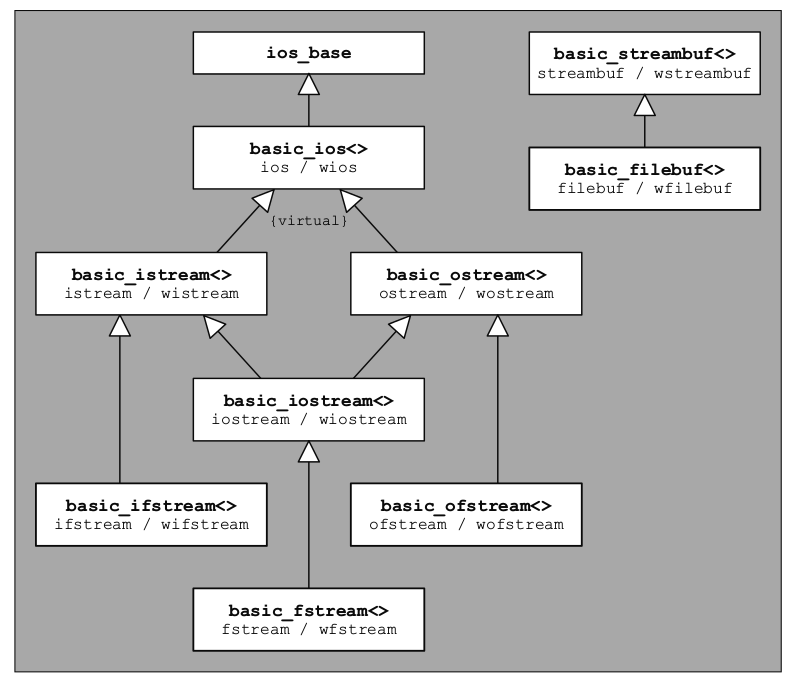
\includegraphics[keepaspectratio,width=0.4\paperwidth]{Pictures/CppStdFileStream.png}
		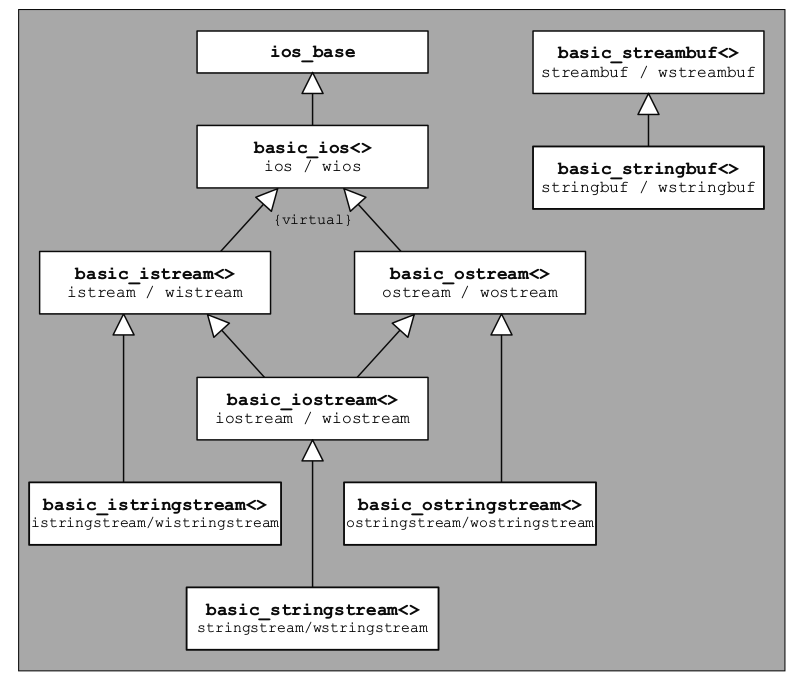
\includegraphics[keepaspectratio,width=0.4\paperwidth]{Pictures/CppStdStringStream.png}
	\caption{文件流与字符流}
	\label{fig:CppStdIoStreams}
	\end{center}
\end{figure}

\verb$ios_base$类是标准IO库类层次的始祖,其派生出\verb$basic_ios$模板类,进而派生其他诸多模板类。
\begin{lstlisting}[language=C++]
typedef basic_ios<char> ios;
typedef basic_istream<char> istream;
typedef basic_ostream<char> ostream;
typedef basic_iostream<char> iostream;
typedef basic_ifstream<char> ifstream;
typedef basic_ofstream<char> ofstream;
typedef basic_fstream<char> fstream;
typedef basic_istringstream<char> istringstream;
typedef basic_ostringstream<char> ostringstream;
typedef basic_stringstream<char> stringstream;
\end{lstlisting}




\clearpage

\subsection{C 块读入}
\begin{lstlisting}[language=C++]
size_t fread (void * ptr, size_t size, size_t count, FILE *stream);
\end{lstlisting}
执行成功时fread返回值应该等于count,注意不是读入的字节数。如果小于count,说明遭遇了出错或eof,与fgetc类似。

下面的程序将一个文件读入内存:
\begin{lstlisting}[language=C++]
/* fread example: read an entire file */
#include <stdio.h>
#include <stdlib.h>

int main () {
    FILE * pFile;
    long lSize;
    char * buffer;
    size_t result;

    pFile = fopen ( "myfile.bin" , "rb" );
    if (pFile==NULL) {fputs ("File error",stderr); exit (1);}

    // obtain file size:
    fseek (pFile , 0 , SEEK_END);
    lSize = ftell (pFile);
    rewind (pFile);

    // allocate memory to contain the whole file:
    buffer = (char*) malloc (sizeof(char)*lSize);
    if (buffer == NULL) {fputs ("Memory error",stderr); exit (2);}

    // copy the file into the buffer:
    result = fread (buffer,1,lSize,pFile);
    if (result != lSize) {fputs ("Reading error",stderr); exit (3);}

    /* the whole file is now loaded in the memory buffer. */

    // terminate
    fclose (pFile);
    free (buffer);
    return 0;
}

\end{lstlisting}

\subsection{C语言的IO流错误}
feof,ferror分别检查文件流的eof指示位和error指示位,返回布尔值。
perror检查errno变量,打印出对应的描述性文字,可以配置打印前缀。
\begin{lstlisting}[language=C]
//stdio.h
int feof(FILE *stream);
int ferror(FILE *stream);
void perror(const char *str);
\end{lstlisting}



以下例子说明了feof的用法:
\begin{lstlisting}[language=C++]
/* feof example: byte counter */
#include <stdio.h>

int main ()
{
    FILE * pFile;
    int n = 0;
    pFile = fopen ("myfile.txt","rb");
    if (pFile==NULL) perror ("Error opening file");
    else
    {   
        while (fgetc(pFile) != EOF) {
            ++n;
        }   
        if (feof(pFile)) {
            puts ("End-of-File reached.");
            printf ("Total number of bytes read: %d\n", n); 
        }   
        else puts ("End-of-File was not reached.");
        fclose (pFile);
    }   
    return 0;
}
\end{lstlisting} 

这个例子说明了ferror的用法:
\begin{lstlisting}[language=C++]
/* ferror example: writing error */
#include <stdio.h>
int main ()
{
    FILE * pFile;
    pFile=fopen("myfile.txt","r");
    if (pFile==NULL) perror ("Error opening file");
    else {
        fputc ('x',pFile);
        if (ferror (pFile))
            printf ("Error Writing to myfile.txt\n");
        fclose (pFile);
    }   
    return 0;
}
\end{lstlisting} 



\subsection{C++ IO流出错状态}
\begin{lstlisting}[language=C++]
//Range relations: bad < fail = operator! < good

std::ios::fail();//Check whether either failbit or badbit is set
std::ios::eof();//Check whether eofbit is set
std::ios::bad();//Check whether badbit is set

//Returns true if none of the stream's error state 
//flags (eofbit, failbit and badbit) is set.
std::ios::good();

//Returns whether an error flag is set (either failbit or badbit).
//Notice that this function does not return the same as member good(), 
//but the opposite of member fail(). 
std::ios::operator bool();
\end{lstlisting}










